\input{../preamble.tex}

\lecturenumber{4}
\title{Kernel (con'd) \\Libraries\\Process}
\version{2.0.0}

\begin{document}
  \begin{frame}[plain, noframenumbering]
    \titlepage
  \end{frame}

\begin{slide}
  
	\slidetitle{You Can Think of the Kernel as a Long Running Process}

	Writing kernel code is more like writing library code
	(there's no \texttt{main})
	\bigskip

	The kernel lets you load code (called modules) which extends core kernel functionality
	\medskip

\end{slide}

\begin{slide}

	\slidetitle{Aside: Function Pointer in C Struct}

	\vspace{-5mm}
	
\begin{minted}{c}
// Called when USB device is plugged in
static int usb_probe(struct usb_interface *interface, const struct usb_device_id *id) {
    printk(KERN_INFO "USB Device Plugged In: Vendor ID=%04X, Product ID=%04X\n",
           id->idVendor, id->idProduct);
    return 0;
}
// Register USB driver with the kernel
static struct usb_driver usb_driver = {
    .name = "example_usb_driver",
    .id_table = usb_table,
    .probe = usb_probe,
    .disconnect = usb_disconnect,
};
// Module Init
static int __init usb_driver_init(void) {
    return usb_register(&usb_driver);
}
\end{minted}

\end{slide}

\begin{slide}
  
  \slidetitle{A Monolithic Kernel Runs Operating System Services in Kernel
              Mode}

  \begin{tikzpicture}[box/.style={draw, minimum width=3.5cm,
                                  minimum height=2em,
                                  inner sep=0.5em, node distance=0.5cm}]
    \draw [blue, dashed, thick] (0,0) -- ($(\textwidth - 3pt, 0)$);
    \node [blue, anchor=south east] at ($(\textwidth - 3pt, 0)$)
          (user) {User space};
    \node [blue, anchor=north east] at ($(\textwidth - 3pt, 0)$)
          (kernel) {Kernel space};
    \node [box] (sched) at ($(\textwidth/2 - 1.5pt, -1.25)$)
          {Process Scheduling};
    \node [box, left=of sched] {Virtual Memory};
    \node [box, right=of sched] {IPC};
    \node [box, below=of sched] (dd) {Device Drivers};
    \node [box, left=of dd] {File Systems};
  \end{tikzpicture}
\end{slide}

\begin{slide}
  
  \slidetitle{A Microkernel Runs the Minimum Amount of Services in Kernel
              Mode}

  \begin{tikzpicture}[box/.style={draw, minimum width=3.5cm,
                                  minimum height=2em,
                                  inner sep=0.5em, node distance=0.5cm}]
    \draw [blue, dashed, thick] (0,0) -- ($(\textwidth - 3pt, 0)$);
    \node [blue, anchor=south east] at ($(\textwidth - 3pt, 0)$)
          (user) {User space};
    \node [blue, anchor=north east] at ($(\textwidth - 3pt, 0)$)
          (kernel) {Kernel space};
    \node [box] (sched) at ($(\textwidth/2 - 1.5pt, -1.25)$)
          {Process Scheduling};
    \node [box, left=of sched] {Virtual Memory};
    \node [box, right=of sched] {Basic IPC};
    \node [box] (dd) at ($(\textwidth/2 - 1.5pt, 1.25)$) {Device Drivers};
    \node [box, left=of dd] {File Systems};
    \node [box, right=of dd] {Advanced IPC};
  \end{tikzpicture}
\end{slide}

\begin{slide}
  
  \slidetitle{Other Types of Kernels}

  ``Hybrid'' kernels are between monolithic and microkernels

  \leftspace{}Emulation services to user mode (Windows)

  \leftspace{}Device drivers to user mode (macOS)
  \bigskip

  Nanokernels and picokernels

  \leftspace{}Move even more into user mode than traditional microkernels
  \bigskip

  There's different architectural lines you can draw with different trade-offs
\end{slide}

  \begin{slide}
    
    \slidetitle{What is an Operating System?}

    The kernel is part of an operating system, but what else?
    \bigskip

    Are macOS, iOS, iPadOS, watchOS, and tvOS all different operating systems?
  \end{slide}

  \begin{slide}
    \slidetitle{Applications May Pass Through Multiple Layers of Libraries}

    \begin{tikzpicture}[box/.style={draw, minimum width=3.5cm, minimum height=2em,
                                    inner sep=0.5em, node distance=0.5cm}]
      \draw [pantone633, dashed, thick] (0,0) -- ($(\textwidth - 3pt, 0)$);
      \node [pantone633, anchor=south east] at ($(\textwidth - 3pt, 0)$)
            (user) {User space};
      \node [pantone633, anchor=north east] at ($(\textwidth - 3pt, 0)$)
            (kernel) {Kernel space};

      \node [box, align=center, minimum width=9.2cm, xshift=-1cm] (libc) at ($(\textwidth/2 - 3pt, 1)$)
            {C Standard Library (libc)};

      \node [box, align=center, above=of libc, anchor=east, xshift=-0.1cm]
            {System Daemon (udev)};

      \node [box, align=center, above=of libc.north east, anchor=east, minimum width=4.5cm]
            (display) {Display Server (Wayland)};

      \node [box, above=of display.north east, anchor=east]
            {GUI Toolkit (GTK)};

      \node [box, fill=black!12.5,anchor=west] (app1) at (0, 5)
            {NetworkManager};

      \node [box, fill=black!12.5, right=of app1] (app2) {LibreOffice};

      \node [box, fill=black!12.5, right=of app2] {Firefox};
    \end{tikzpicture}
  \end{slide}

  \begin{slide}

    \slidetitle{What an Operating System is Depends on the Application}

    Android and Debian both use the Linux kernel,
    
    \leftspace{}but the applications are different
    \medskip

    Maybe they're the same OS if you only care about terminal applications
    \bigskip

    ``Linux'' distributions may be considered GNU/Linux

    \leftspace{}GNU distributes the standard C library and common utilities
    \bigskip

    An OS consists of a kernel and libraries required for your
    application
  \end{slide}


\begin{slide}

\slidetitle{Normal Compilation in C}

	\begin{center}
	\begin{tikzpicture}[>=stealth', shorten >=2pt]
	  \node[draw, align=left] (main) {\texttt{main.c}};
	  \node[draw, align=left, below=of main, yshift=1em] (util)
		   {\texttt{util.c}};
	  \node[draw, align=left, below=of util, yshift=1em] (foo)
		   {\texttt{foo.c}};
	  \node[draw, align=left, below=of foo, yshift=1em] (bar)
		   {\texttt{bar.c}};

	  \node[draw, align=left, right=of main, xshift=6em] (main-obj)
		   {\texttt{main.o}};
	  \node[draw, align=left, below=of main-obj, yshift=1em] (util-obj)
		   {\texttt{util.o}};
	  \node[draw, align=left, below=of util-obj, yshift=1em] (foo-obj)
		   {\texttt{foo.o}};
	  \node[draw, align=left, below=of foo-obj, yshift=1em] (bar-obj)
		   {\texttt{bar.o}};

	  \node[draw, align=left, right=of main-obj, xshift=6em] (exec)
		   {\texttt{executable}};

	  \draw[->] (main) -- node [above] {\small Compilation} (main-obj);
	  \draw[->] (util) -- (util-obj);
	  \draw[->] (foo) -- (foo-obj);
	  \draw[->] (bar) -- (bar-obj);
	  \draw[->] (main-obj) -- node [above] {\small Linkage} (exec);
	  \draw[->] (util-obj) -- (exec);
	  \draw[->] (foo-obj) -- (exec);
	  \draw[->] (bar-obj) -- (exec);
	\end{tikzpicture}
	\end{center}

	\vspace{1em}

	Note: object files (\texttt{.o}) are just ELF files with code for functions
	
\end{slide}

  \begin{slide}
    
    \slidetitle{Static Libraries Are Included At Link Time}

    \begin{tikzpicture}[shorten >=3pt]
      \node[draw, align=left] (util-obj)
           {\texttt{util.o}};
      \node[draw, align=left, below=of util-obj, yshift=1em] (foo-obj)
           {\texttt{foo.o}};
      \node[draw, align=left, below=of foo-obj, yshift=1em] (bar-obj)
           {\texttt{bar.o}};

      \node[draw, align=left, right=of util-obj, xshift=6em] (static)
           {\texttt{lib.a}};

      \draw[->] (util-obj) -- node [above] {\small Archive} (static);
      \draw[->] (foo-obj) -- (static);
      \draw[->] (bar-obj) -- (static);
    \end{tikzpicture}

    \begin{flushright}
    \begin{tikzpicture}[>=stealth', shorten >=2pt]

      \node[draw, align=left] (main-obj)
           {\texttt{main.o}};
      \node[draw, align=left, below=of main-obj, yshift=1em] (static)
           {\texttt{lib.a}};

      \node[draw, align=left, right=of main-obj, xshift=6em] (exec)
           {\texttt{executable}};

      \draw[->] (main-obj) -- node [above] {\small Linkage} (exec);
      \draw[->] (static) -- (exec);
    \end{tikzpicture}
    \end{flushright}
  \end{slide}

  \begin{slide}
    
    \slidetitle{Dynamic Libraries Are For Reusable Code}

    The C standard library is a dynamic library (\texttt{.so}), like any other
    on the system

    \leftspace{} Basically a collection of \texttt{.o} files containing function
    definitions
    \bigskip

    Multiple applications can use the same library:
    \medskip

    \begin{tikzpicture}[>=stealth', shorten >=2pt]
      \node[draw] (app1) {Application 1};
      \node[draw, right=of app1] (app2) {Application 2};
      \node[draw, below=of app1, xshift=5em] (libc) {\texttt{libc.so}};
      \draw[->] (app1) -- (libc);
      \draw[->] (app2) -- (libc);
    \end{tikzpicture}
    \medskip

    The operating system only loads \texttt{libc.so} in memory once, and shares
    it
  \end{slide}

  \begin{slide}
    
    \slidetitle{Dynamic Libraries Are Included At Runtime}

    \begin{tikzpicture}[shorten >=3pt]
      \node[draw, align=left] (util-obj)
           {\texttt{util.o}};
      \node[draw, align=left, below=of util-obj, yshift=1em] (foo-obj)
           {\texttt{foo.o}};
      \node[draw, align=left, below=of foo-obj, yshift=1em] (bar-obj)
           {\texttt{bar.o}};

      \node[draw, align=left, right=of util-obj, xshift=6em] (static)
           {\texttt{lib.so}};

      \draw[->] (util-obj) -- node [above] {\small Shared Linkage} (static);
      \draw[->] (foo-obj) -- (static);
      \draw[->] (bar-obj) -- (static);
    \end{tikzpicture}

    \begin{flushright}
    \begin{tikzpicture}[>=stealth', shorten >=2pt]

      \node[draw, align=left] (main-obj)
           {\texttt{main.o}};

      \node[draw, align=left, right=of main-obj, xshift=6em] (exec)
           {\texttt{executable}};

      \node[draw, align=left, below=of exec, yshift=1em] (dynamic)
           {\texttt{lib.so}};

      \draw[->] (main-obj) -- node [above] {\small Linkage} (exec);
      \draw[->] (exec) -- node [right] {\small Linked at Runtime} (dynamic);
    \end{tikzpicture}
    \end{flushright}
  \end{slide}

  \begin{slide}

    \slidetitle{Useful Command Line Utility for Dynamic Libraries}

    \texttt{ldd <executable>}
    
    \leftspace{}shows which dynamic libraries an executable uses
  \end{slide}

  \begin{slide}
    \slidetitle{Static vs Dynamic Libraries}

    To statically link your code

    \leftspace{}Basically copies the \texttt{.o} files directly into the
    executable
    \bigskip

    The drawbacks compared to dynamic libraries:
    \begin{itemize}
      \item Statically linking prevents re-using libraries
      
            (commonly used libraries have many duplicates)
      \item Any updates to a static library requires the executable to be
            recompiled
    \end{itemize}
    \bigskip

    What are issues with dynamic libraries?
  \end{slide}

\begin{slide}

	\slidetitle{Program and Process}
	
	A \textbf{program} consists of static code and data, e.g., on the disk.
	\bigskip
	
	A \textbf{process} is an instance of a program (at any time there may be 0 or
	more instances of a program running, e.g., a user may run multiple concurrent
	shells).
  
\end{slide}

\begin{slide}

	\slidetitle{Process Creation}
	
	\vspace{-5mm}
	\resizebox{0.5\textwidth}{0.5\textwidth}{%
	
		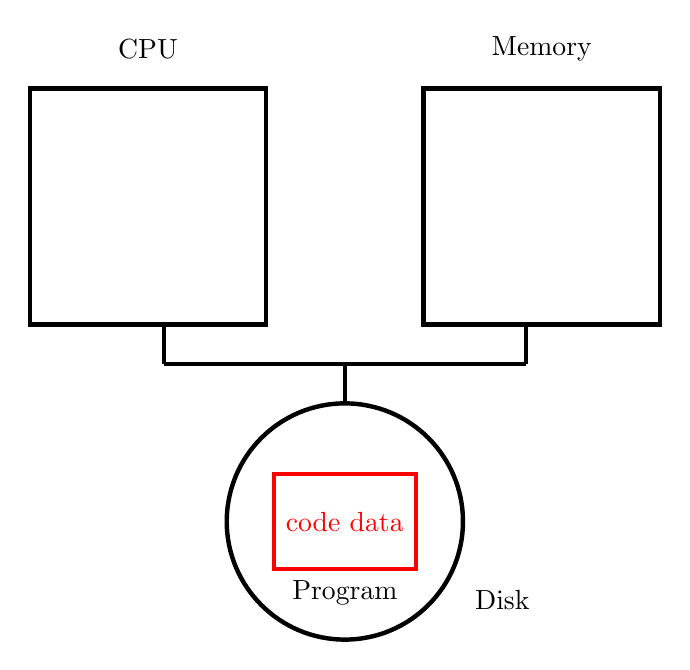
\begin{tikzpicture}

		\node at (0,5) {CPU};
		\node (A) at (0,3) [draw,ultra thick,minimum width=3cm, minimum height=3cm] {};
		\node at (5,5) {Memory};
		\node (B) at (5,3) [draw,ultra thick,minimum width=3cm, minimum height=3cm] {};

		\node at (4.5,-2) {Disk};
		\draw (2.5,-1) [ultra thick] circle (1.5cm);

		\node at (2.5,-1.9) {Program};
		\node at (2.5,-1) [red,draw,ultra thick, text width=1.5cm, minimum width=1.8cm,
		minimum height=1.2cm] {code data};

		\draw [ultra thick] (0.2, 1) -- (4.8, 1);
		\draw [ultra thick] (0.2, 1) -- (0.2, 1.5);
		\draw [ultra thick] (4.8, 1) -- (4.8, 1.5);
		\draw [ultra thick] (2.5, 1) -- (2.5, 0.5);


		\end{tikzpicture}
	}
	
\end{slide}

\begin{slide}

	\slidetitle{A Process Control Block (PCB) Contains All Information}

	Specifically, in Linux, this is the \texttt{\color{blue}
	task\_struct} you can browse on

	\href{https://github.com/torvalds/linux/blob/master/include/linux/sched.h\#L743}
		 {GitHub}
	\medskip

	It contains:
	\begin{itemize}
	  \item Process ID (PID)
	  \item Process state
	  \item CPU registers
	  \item Scheduling information
	  \item Memory management information
	  \item I/O status information
	  \item Any other type of accounting information
	\end{itemize}
	\medskip

	Each process gets a unique process ID (pid) to keep track of it

\end{slide}
	
\begin{slide}

	\slidetitle{Process Creation}
	
	\vspace{-5mm}
	\resizebox{0.5\textwidth}{0.5\textwidth}{%

		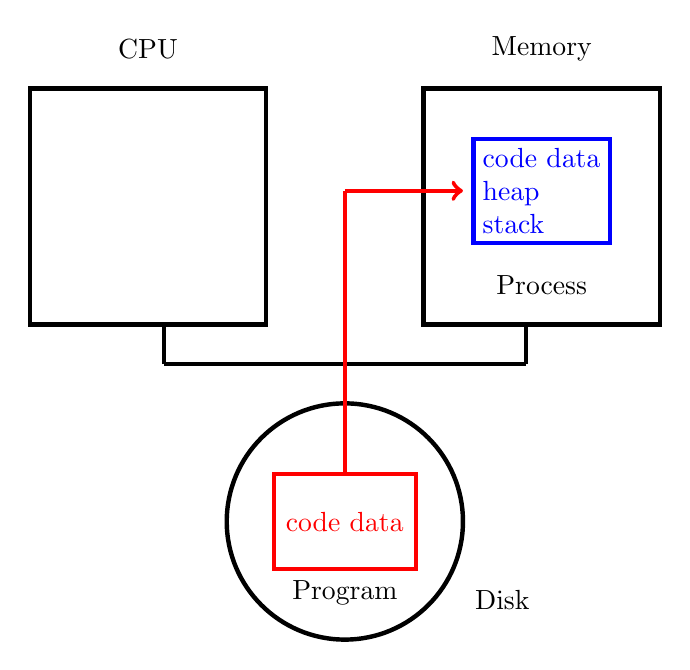
\begin{tikzpicture}

		\node at (0,5) {CPU};
		\node (A) at (0,3) [draw,ultra thick,minimum width=3cm, minimum height=3cm] {};
		\node at (5,5) {Memory};
		\node (B) at (5,3) [draw,ultra thick,minimum width=3cm, minimum height=3cm] {};

		\node at (4.5,-2) {Disk};
		\draw (2.5,-1) [ultra thick] circle (1.5cm);

		\node at (2.5,-1.9) {Program};
		\node (PRG) at (2.5,-1) [red,draw,ultra thick, text width=1.5cm, minimum width=1.8cm,
		minimum height=1.2cm] {code data};

		\node at (5,2) {Process};
		\node (PRC) at (5,3.2) [blue,draw,ultra thick, text width=1.5cm, minimum width=1.5cm,
		minimum height=1.2cm] {code data heap stack};

		\draw [ultra thick] (0.2, 1) -- (4.8, 1);
		\draw [ultra thick] (0.2, 1) -- (0.2, 1.5);
		\draw [ultra thick] (4.8, 1) -- (4.8, 1.5);
		\draw [ultra thick] (2.5, 1) -- (2.5, 0.5);


		\draw [ultra thick, red] (2.5, -0.4) -- (2.5, 3.2);
		\draw [ultra thick, red, ->] (2.5, 3.2) -- (4, 3.2);

		\end{tikzpicture}
	}

\end{slide}

\begin{slide}

	\slidetitle{Process Creation}
	
	OS allocates internal data structures (PCB)
	\bigskip
	
	OS allocates an address space
    \bigskip
	
	OS opens basic files (STDIN, STDOUT, STDERR)
	\bigskip
	
	OS initializes CPU registers
	\bigskip

\end{slide}

\begin{slide}

	\slidetitle{Program, Process, Thread}
	
	A \textbf{program} is on-disk application, consisting of code and data; programs become a process when they are executed
	\bigskip
	
    A \textbf{process} is a running instance of a program. A process starts with a single thread of execution and an address space.
	\bigskip
	
    A process can launch multiple \textbf{threads} of execution in the same address space. Each thread receives its own stack but they share global data, code, and heap.
	
\end{slide}

\begin{slide}
	
	\slidetitle{Running Processes On My Laptop}
	
	\centering
	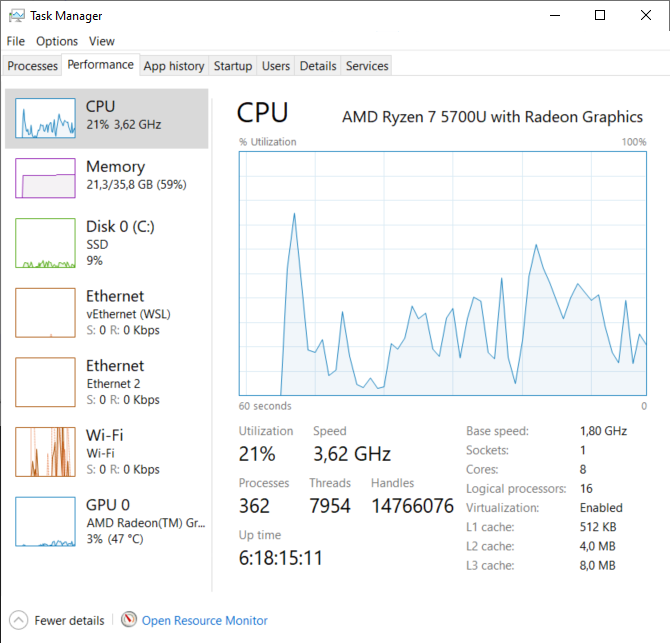
\includegraphics[width=60mm]{windows_num_process.png}
		
\end{slide}

\begin{slide}

	\slidetitle{Sharing Resources}
	
	\vspace{-5mm}
	
	\begin{minipage}[t]{0.45\textwidth}
	\vspace{0pt}\par
	\centering
		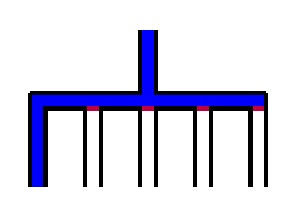
\begin{tikzpicture}
		\fill [blue] (1.4,1) rectangle (1.6,0.2);
		\fill [blue] (0,0) rectangle (3,0.2);

		\draw [ultra thick, purple] (0.2,0) -- (3,0);

		\fill [blue] (0,0) rectangle (0.2,-1);


		\draw [ultra thick, black] (0,0.2) -- (1.4,0.2) -- (1.4,1);
		\draw [ultra thick, black] (1.6,1) -- (1.6,0.2) -- (3,0.2);
		\draw [ultra thick, black] (0,0.2) -- (0,-1);
		\draw [ultra thick, black] (3,0.2) -- (3,-1);
		\draw [ultra thick, black] (0.2,-1) -- (0.2,0) -- (0.7,0) -- (0.7,-1);
		\draw [ultra thick, black] (0.9,-1) -- (0.9,0) -- (1.4,0) -- (1.4,-1);
		\draw [ultra thick, black] (1.6,-1) -- (1.6,0) -- (2.1,0) -- (2.1,-1);
		\draw [ultra thick, black] (2.3,-1) -- (2.3,0) -- (2.8,0) -- (2.8,-1);

		\end{tikzpicture}

		Time sharing (one at a time)
		
	\end{minipage}
	\hfill
	\begin{minipage}[t]{0.45\textwidth}
	\vspace{0pt}\par
	\centering
		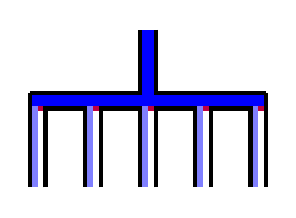
\begin{tikzpicture}
		\fill [blue] (1.4,1) rectangle (1.6,0.2);
		\fill [blue] (0,0) rectangle (3,0.2);

		\draw [ultra thick, purple] (0,0) -- (3,0);

		\fill [blue!50] (0,0.03) rectangle (0.1,-1);
		\fill [blue!50] (0.7,0.03) rectangle (0.8,-1);
		\fill [blue!50] (1.4,0.03) rectangle (1.5,-1);
		\fill [blue!50] (2.1,0.03) rectangle (2.2,-1);
		\fill [blue!50] (2.8,0.03) rectangle (2.9,-1);

		\draw [ultra thick, black] (0,0.2) -- (1.4,0.2) -- (1.4,1);
		\draw [ultra thick, black] (1.6,1) -- (1.6,0.2) -- (3,0.2);
		\draw [ultra thick, black] (0,0.2) -- (0,-1);
		\draw [ultra thick, black] (3,0.2) -- (3,-1);
		\draw [ultra thick, black] (0.2,-1) -- (0.2,0) -- (0.7,0) -- (0.7,-1);
		\draw [ultra thick, black] (0.9,-1) -- (0.9,0) -- (1.4,0) -- (1.4,-1);
		\draw [ultra thick, black] (1.6,-1) -- (1.6,0) -- (2.1,0) -- (2.1,-1);
		\draw [ultra thick, black] (2.3,-1) -- (2.3,0) -- (2.8,0) -- (2.8,-1);

		\end{tikzpicture}

		Space sharing (all a little)
		
	\end{minipage}

\end{slide}
	
\begin{slide}

	\slidetitle{Virtualizing the CPU}
	
	Goal: give each process the illusion of exclusive CPU access
	\medskip
	
	Reality: the CPU is a shared resource among all processes
	\bigskip
	
\end{slide}

\begin{slide}

	\slidetitle{OS provides process abstraction}
	
	When the user executes a program, the OS creates a process
	\bigskip
	
	OS time-shares CPU across multiple processes
	\bigskip
	
	OS scheduler picks one of the executable processes to run
	
\end{slide}

\begin{slide}
	\slidetitle{Process State Diagram (You Could Rename Waiting to Ready)}

	\begin{tikzpicture}[
	  every initial by arrow/.style={rawarrow},
	  every state/.style={ellipse, minimum width=2.5cm, minimum height=1cm, font=\small},
	]
	  \node [state, initial] (created) {Created};
	  \node [state, right=of created] (waiting) {Waiting};
	  \node [state, above right=of waiting] (running) {Running};
	  \node [state, below right=of waiting] (blocked) {Blocked};
	  \node [state, accepting, below right=of running] (terminated) {Terminated};
	  \path [rawarrow] (created) edge (waiting)
				 (waiting) edge [bend left] (running)
				 (running) edge [bend left] (waiting)
				 (running) edge (blocked)
				 (blocked) edge (waiting)
				 (running) edge (terminated);
	\end{tikzpicture}
\end{slide}

\begin{slide}

	\slidetitle{Process State Transitions}

	\vspace{-3mm}
	
	Process 0 takes 5 timesteps to complete
	
	Process 0 initiates I/O after 3 time steps (takes 4 time steps)
	
	Process 1 takes 5 timesteps to complete
	
	Process State Transitions: Running Until Blocked or Completion 
	
	\bigskip
	
	\centering
	\begin{tabular}{rllp{5cm}}
		\textbf{Time} & \textbf{Process 0} & \textbf{Process 1} & \textbf{Notes} \\
		1  & Running   & Ready     &  \\
		2  &    &      &  \\
		3  &    &      &  \\
		4  &    &    &  \\
		5  &    &    &  \\
		6  &    &    &  \\
		7  &    &    &  \\
		8  &      &    &  \\
		9  &    &          &  \\
	\end{tabular}

\end{slide}

\begin{slide}

	\slidetitle{Process State Transitions}

	\vspace{-3mm}
	
	Process 0 takes 5 timesteps to complete
	
	Process 0 initiates I/O after 3 time steps (takes 4 time steps)
	
	Process 1 takes 5 timesteps to complete
	
	Process State Transitions: Switch after running 2 timesteps 
	
	\bigskip
	
	\centering
	\begin{tabular}{rllp{5cm}}
		\textbf{Time} & \textbf{Process 0} & \textbf{Process 1} & \textbf{Notes} \\
		1  & Running   & Ready     &  \\
		2  &    &      &  \\
		3  &    &      &  \\
		4  &    &    &  \\
		5  &    &    &  \\
		6  &    &    &  \\
		7  &    &    &  \\
		8  &      &    &  \\
		9  &    &          &  \\
	\end{tabular}

\end{slide}

\begin{slide}

	\slidetitle{Draw the Process Structure}

\end{slide}

\end{document}
